\documentclass[../main.tex]{subfiles}

\begin{document}
\chapter{Differentialrechnung}\label{chp:differential}
Dieses Kapitel stellt den Hauptteil dieser Vorlesung dar.
Auch in~\cite{heuser} ist das korrespondierende
Kapitel XX bei weitem das grösste. Der Inhalt ist das
Studium differenzierbarer Abbildungen 
$f \colon \mathbb{R}^m \to \mathbb{R}^n$.
Die erste Schwierigkeit daran ist, dass der Ausdruck
\[
  \lim_{h \to 0} \frac{f(p + h) - f(p)}{h}
\]
für $m \geq 2$ keinen Sinn macht: Vektoren kann man nicht
definieren.

\section{Differenzierbarkeit}
\begin{definition}
  Sei $U \subset \mathbb{R}^m$ offen. Eine Abbildung
  $f \colon U \to \mathbb{R}^n$ heisst
  \emph{differenzierbar} im Punkt $p \in U$, falls
  folgendes existiert:
  \begin{enumerate}[(i)]
    \item eine lineare Abbildung 
      ${(Df)}_p \colon \mathbb{R}^m \to \mathbb{R}^n$,
      genannt \emph{Differential} von $f$ an
      der Stelle $p$,
    \item für alle $h \in \mathbb{R}^m$ mit $p + h \in U$ 
      ein \emph{Restterm} ${(Rf)}_p(h) \in \mathbb{R}^n$,
      der relativ klein in $\Vert h \Vert_2$ ist,
      so dass für alle $h \in \mathbb{R}^m$ mit $p + h \in U$ 
      gilt, dass
      \[
        f(p+h) = f(p) + {(Df)}_p(h) + {(Rf)}_p(h).
      \]
  \end{enumerate}
  Der Unterteilung von $f$ in diese drei Summanden sagt man
  \emph{Dreigliedentwicklung}. Die Forderung,
  dass ${(Rf)}_p(h)$ \emph{relativ klein} in $\Vert h \Vert_2$ 
  ist, bedeutet, dass
  \[
    \lim_{h \to 0} \frac{\Vert {(Rf)}_p(h)\Vert_2}{\Vert h \Vert_2}
    = 0.
  \]
  In anderen Worten existiert für alle $\varepsilon > 0$ ein $\delta > 0 $,
  so dass für alle $h \in \mathbb{R}^m$ mit $\Vert h \Vert_2
  \leq \delta$ gilt, dass $\Vert {(Rf)}_p(h) \Vert_2
  \leq \varepsilon \cdot \Vert h \Vert_2$.
\end{definition}

\begin{remark}
  Das Differential ist a priori nur für diejenigen
  $h$ definiert, für die $p + h$ noch in $U$ 
  liegt. Da $U$ aber offen ist, existiert aber
  eine Basis von $\mathbb{R}^m$ aus Vektoren
  $h_i$ für die $p + h_i$ noch in $U$ liegt.
  Da lineare Abbildungen durch die Bilder der
  Basisvektoren eindeutig bestimmt sind, lässt
  sich das Differential auf ganz $\mathbb{R}^m$
  erweitern.
\end{remark}

\begin{example}
  Sei $L \colon \mathbb{R}^m \to \mathbb{R}^n$ linear.
  Dann gilt für alle $p, h \in \mathbb{R}^m$,
  dass
  \[
    L(p + h) = L(p) + L(h).
  \]
  Dies ist eine Dreigliedentwicklung für $L$ 
  an der Stelle $p$ mit Restterm ${(RL)}_p(h) = 0$.
  Tatsächlich ist die Abbildung ${(DL)}_p = L$ linear.
  Die informale Erklärung dafür ist,
  dass~$L$ die ``beste lineare Approximation'' von $L$ 
  ist, und das an jeder Stelle.
\end{example}

\begin{examples}
  \leavevmode
  \begin{enumerate}[(1)]
    \item Betrachte die Funktion
      \begin{align*}
        f \colon \mathbb{R}^m & \to \mathbb{R} \\
        p & \mapsto \langle p, p \rangle.
      \end{align*}
      Für alle $p, h \in \mathbb{R}^m$ gilt, dass
      \[
        f(p+ h) = \langle p + h, p + h \rangle
        = \langle p, p \rangle + 2 \langle p, h \rangle + \langle h, h \rangle.
      \]
      Dies ist eine Dreigliedentwicklung für $f$ mit
      Differential
      ${(Df)}_p(h) = 2 \langle p, h \rangle$ und
      Restterm
      ${(Rf)}_p(h) = \langle h, h \rangle$.
      Tatsächlich ist ${(Df)}_p$ linear in $h$,
      da Skalarprodukte bilinear sind, und
      \[
        {(Rf)}_p(h) = \langle h, h \rangle = \Vert h \Vert_2^2
      \]
      ist relativ klein in $\Vert h \Vert_2$.
      Zum Beweis dafür sei $\varepsilon > 0$ und setze
      $\delta = \varepsilon$.
      Für alle $h \in \mathbb{R}^m$ mit $\Vert h \Vert_2 \leq \delta$ 
      gilt dann, dass
      \(
        |{(Rf)}_p(h)| = \Vert h \Vert_2^2 \leq \varepsilon \cdot \Vert h \Vert_2
      \).
    \item Betrachte die Abbildung
      \begin{align*}
        m \colon \mathbb{R}^2 & \to \mathbb{R} \\
        (x, y) & \mapsto xy.
      \end{align*}
      Seien $p = (p_1, p_2)$ und $h = (h_1, h_2)$ in $\mathbb{R}^2$.
      Dann gilt
      \[
        m(p + h) = (p_1 + h_1) \cdot (p_2 + h_2)
        = p_1 p_2 + (p_1 h_2 + p_2 h_1) + h_1 h_2.
      \]
      Dies ist eine Dreigliedentwicklung für $m$ bei $p$
      mit ${(Dm)}_p(h) = p_1 h_2 + p_2 h_1$ und
      ${(Rm)}_p(h) = h_1 h_2$.
      Da
      \[
        {(Dm)}_p(h) =
        \begin{pmatrix}
          p_2 & p_1
        \end{pmatrix}
        \begin{pmatrix}
          h_1 \\ h_2
        \end{pmatrix}
      \]
      gilt, ist ${(Dm)}_p$ linear.
      Weiter ist der Restterm 
      relativ klein in $\Vert h \Vert_2$, da
      \[
        |{(Rm)}_p(h)| = |h_1| \cdot |h_2| \leq \Vert h \Vert_2 \cdot
        \Vert h \Vert_2 = \Vert h \Vert_2^2,
      \]
      und $\Vert h \Vert_2^2$ ist nach Beispiel (1)
      relativ klein in $\Vert h \Vert_2$.
  \end{enumerate}
\end{examples}

Wir treffen nun die Kettenregel als Quelle
für viele Beispiele an.
Wir werden sie später in diesem Kapitel beweisen.

\begin{theorem*}[Kettenregel]
  Seien $U \subset \mathbb{R}^m$ und $V \subset \mathbb{R}^k$ 
  offen, und sei $f \colon U \to \mathbb{R}^k$ differenzierbar
  bei $p \in U$ mit $f(U) \subset V$,
  sowie $g \colon V \to \mathbb{R}^n$ bei $f(p) \in V$ 
  differenzierbar.
  Dann ist die Komposition $g \circ f \colon U \to \mathbb{R}^n$ 
  differenzierbar bei $p$, und es gilt
  \[
    {(D(g \circ f))}_p = {(Dg)}_{f(p)} \circ {(Df)}_p.
  \]
\end{theorem*}

\begin{example}
  Betrachte die Abbildung
  \begin{align*}
    \ell \colon \mathbb{R}^m & \to \mathbb{R} \\
    p & \mapsto \sqrt{\langle p, p \rangle}.
  \end{align*}
  In Koordinaten $x_1, \dots, x_m$ ist
   \[
     \ell(x_1, \dots, x_m) = \sqrt{x_1^2 + \cdots + x_m^2}.
  \]
  Sei $U = \mathbb{R}^m \setminus \{0\} \subset \mathbb{R}^m$ 
  und $V = \mathbb{R}_{>0}$.
  Beide dieser Mengen sind offen. Setze weiterhin
  \begin{align*}
    f \colon U & \to \mathbb{R} \\
    p & \mapsto \langle p, p \rangle
  \end{align*}
  und
  \begin{align*}
    g \colon \mathbb{R}_{>0} & \to \mathbb{R} \\
    t & \mapsto \sqrt t.
  \end{align*}
  Für alle $p \in U$ gilt $\ell(p) = g(f(p))$.
  Die Funktion $f$ ist differenzierbar in allen
  Punkten $p \in U$ 
  (eigentlich sogar in allen $p \in \mathbb{R}^n$).
  Ausserdem ist $g$ differenzierbar an allen Stellen
  $t > 0$.
  Aus der Analysis I wissen wir, dass
  \[
    {(Dg)}_t(h) = g'(t) \cdot h = \frac{1}{2 \sqrt t} \cdot h.
  \]
  Die Kettenregel liefert, dass
  $\ell = g \circ f$ an jeder Stelle $p \in U$ differenzierbar ist,
  und es gilt
  \[
    {(D \ell)}_p(h) = {(Dg)}_{f(p)}({(Df)}_p(h))
    = \frac{1}{2 \sqrt{\langle p, p \rangle}} \cdot 2 \langle p, h \rangle
    = \langle p / \Vert p \Vert_2, h \rangle.
  \]
  Der Vektor $p / \Vert p \Vert_2$ ist der Vektor mit Länge $1$,
  der in die selbe Richtung zeigt wie $p$.
  Er beschreibt den ``Zuwachs'' der Funktion $\ell$.
\end{example}

\begin{definition}
  Sei $f \colon \mathbb{R}^m \to \mathbb{R}^n$ eine Abbildung.
  Dann existieren eindeutige \emph{Komponentenfunktionen}
  $f_k \colon R^m \to \mathbb{R}$ 
  für $1 \leq k \leq n$ mit folgender Eigenschaft:
  für alle $p \in \mathbb{R}^m$ gilt, dass
  \[
    f(p) = \sum_{k=1}^{n} f_k(p) \cdot e_k.
  \]
\end{definition}

\begin{lemma*}
  Eine Abbildung $f \colon \mathbb{R}^m \to \mathbb{R}^n$ ist differenzierbar,
  genau dann wenn alle Komponentenfunktionen 
  $f_k \colon \mathbb{R}^m \to \mathbb{R}$ bei $p$ differenzierbar sind.
\end{lemma*}

\begin{proof}
  Um zu zeigen, dass die Komponentenfunktionen einer
  differenzierbaren Abbildung $f \colon \mathbb{R}^m \to \mathbb{R}^n$
  selbst differenzierbar sind, sei
  \[
    f(p + h) = f(p) + {(Df)}_p(h) + {(Rf)}_p(h)
  \]
  eine Dreigliedentwicklung von $f$.
  Für $1 \leq k \leq n$ 
  setze ${(Df_k)}_p(h) = \langle {(Df)}_p(h), e_k \rangle$ 
  und ${(Rf_k)}_p(h) = \langle {(Rf)}_p(h), e_k \rangle$.
  Dann gilt für alle $k \leq n$, dass
  \[
    f_k(p + h) = f_k(p) + {(Df_k)}_p(h) + {(Rf_k)}_p(h).
  \]
  Weiterhin ist
  \begin{enumerate}[(i)]
    \item die Funktion
      \begin{align*}
        {(Df_k)}_p \colon \mathbb{R}^m & \to \mathbb{R} \\
        h & \mapsto \langle {(Df)}_p(h), e_k \rangle
      \end{align*}
      als Verknüpfung einer linearen Funktion mit einer Projektion
      linear,
    \item der Restterm ${(Rf_k)}_p(h)$ relativ klein
      in $\Vert h \Vert_2$, da 
      \(
        |{(Rf_k)}_p(h)| \leq \Vert {(Rf)}_p(h) \Vert_2
      \)
      gilt.
  \end{enumerate}

  Umgekehrt nehmen wir an, dass die Komponentenfunktionen
  $f_k \colon \mathbb{R}^m \to \mathbb{R}$
  einer Funktion $f \colon \mathbb{R}^m \to \mathbb{R}^n$ 
  differenzierbar sind.
  Für alle $k$ gibt es dann eine Dreigliedentwicklung
  \(
    f_k(p + h) = f_k(p) + {(Df_k)}_p(h) + {(Rf_k)}_p(h).
  \)
  Setze
  \[
    {(Df)}_p(h) = \sum_{k=1}^{n} {(Df_k)}_p(h) \cdot e_k
  \]
  und
  \[
    {(Rf)}_p(h) = \sum_{k=1}^{n} {(Rf_k)}_p(h) \cdot e_k.
  \]
  Dann gilt
  \(
    f(p + h) = f(p) + {(Df)}_p(h) + {(Rf)}_p(h).
  \)
  Weiterhin ist
  \begin{enumerate}[(i)]
    \item die Abbildung
      \begin{align*}
        {(Df)}_p \colon \mathbb{R}^m & \to \mathbb{R}^n \\
        h & \mapsto \sum_{k=1}^{n} {(Df_k)}_p(h) \cdot e_k
      \end{align*}
      linear da Summen linearer Abbildungen linear sind, und
    \item ${(Rf)}_p(h)$ ist relativ klein in $\Vert h \Vert_2$,
      da
      \[
        \Vert {(Rf)}_p(h) \Vert_2 \leq \sum_{k=1}^{n} |{(Rf_k)}_p(h)|.
      \]
      Dies folgt aus der allgemeinen Ungleichung, dass
      die euklidische Norm immer kleiner ist als die Summennorm.
      Weiterhin verwenden wir, dass endliche Summen
      relativ kleiner Funktionen selbst relativ klein ist.
      Dazu teile $\varepsilon$ durch $n$ um ein geeignetes
      $\delta$ als Minimum $n$ verschiedener $\delta$ zu bekommen.
      \qedhere
  \end{enumerate}
\end{proof}

\begin{question}
  Können wir die Differenzierbarkeit von Abbildungen
  $f \colon \mathbb{R}^m \to \mathbb{R}$ weiter 
  auf die Differenzierbarkeit von Funktionen
  $g \colon \mathbb{R} \to \mathbb{R}$ zurückführen?
  Konkreter: Ist $f \colon \mathbb{R}^m \to \mathbb{R}$ 
  bei $p = 0$ differenzierbar, falls die Einschränkung
  von $f$ auf allen Koordinatenachsen differenzierbar ist?
\end{question}

Die Antwort hier ist leider ``nein'', wie in folgendem
Beispiel zu erkennen ist.

\begin{example}
  Betrachte die Funktion
  \begin{align*}
    f \colon \mathbb{R}^2 & \to \mathbb{R} \\
    (x, y) & \mapsto 
    \begin{cases}
      \frac{xy}{x^2 + y^2} & (x, y) \neq (0, 0) \\
      0 & (x, y) = (0, 0).
    \end{cases}
  \end{align*}
  Die Einschränkung von $f$ auf beide Achsen ist identisch null,
  also differenzierbar. Aber $f$ ist nicht einmal stetig im Nullpunkt:
  \[
    \lim_{n \to \infty} f(1/n, 1/n) = \frac{1}{2} \neq f(0, 0).
  \]
  Vergleiche auch Serie 6 für ein Beispiel einer Funktion, die
  trotz Stetigkeit im Nullpunkt dort nicht differenzierbar ist.
\end{example}

\begin{remark}
  Falls $f$ an der Stelle $p \in U$ eine
  Dreigliedentwicklung besitzt,
  dann ist diese eindeutig.
  Insbesondere ist das Differential 
  ${(Df)}_p \colon \mathbb{R}^m \to \mathbb{R}^n$ 
  wohldefiniert.
  Der Grund für die Eindeutigkeit des Differentials
  liegt darin, dass nur die Nullfunktion
  gleichzeitig linear und relativ klein ist.
  Man kann zeigen, dass die Differenz
  zweier potentiellen Differentialen derselben Funktion
  diese Eigenschaften erfüllt.
  Die Details dazu werden in Serie 7 behandelt.
\end{remark}

\begin{definition}
  Das Differential ${(Df)}_p \colon \mathbb{R}^m \to \mathbb{R}^n$ 
  einer differenzierbaren Funktion $f$
  ist linear,
  hat also bezüglich der Standardbasen auf
  $\mathbb{R}^m$ und $\mathbb{R}^n$ eine
  Abbildungsmatrix ${(Jf)}_p \in \mathbb{R}^{n \times m}$,
  genannt \emph{Jakobimatrix} von $f$ an der
  Stelle $p \in U$.
\end{definition}

Wir bestimmen nun die Einträge der Jakobimatrix
${(Jf)}_p$.
Schreibe wie üblich
\[
  f(p) = \sum_{k=1}^{n} f_k(p) e_k.
\]
Die Koeffizienten von ${(Jf)}_p$ sind dann
\begin{align*}
  {({(Jf)}_p)}_{ij} 
  &= \langle {(Df)}_p(e_j), e_i \rangle  \\
  &= \left\langle 
    \sum_{k=1}^{n} {(Df_k)}_p(e_j) e_k,
    e_i
  \right\rangle \\
  &= {(Df_i)}_p(e_j).
\end{align*}

\begin{definition}
  Sei $U \subset \mathbb{R}^m$ offen und
  $f \colon U \to \mathbb{R}^n$ differenzierbar.
  Die $j$-te \emph{partielle Ableitung}
  von $f_i \colon \mathbb{R}^m \to \mathbb{R}$ ist
  gegeben durch
  \[
    \frac{\partial f_i}{\partial x_j}(p) = {(Df_i)}_p(e_j) \in \mathbb{R}.
  \]
\end{definition}

Gemäss dieser Definition ist dann
\[
  {(Jf)}_p =
  \begin{pmatrix}
    {\partial f_1}/{\partial x_1}(p)
    & {\partial f_1}/{\partial x_2}(p)
    & \cdots
    &{\partial f_1}/{\partial x_m}(p)
    \\
    {\partial f_2}/{\partial x_1}(p)
    & {\partial f_2}/{\partial x_2}(p)
    & \cdots
    & {\partial f_2}/{\partial x_m}(p)\\
    \vdots & \vdots & \ddots & \vdots \\
    \partial f_n / \partial x_1 (p)
    & \partial f_n / \partial x_2 (p)
    & \cdots
    & \partial f_n / \partial x_m(p)
  \end{pmatrix}.
\]
Im Spezialfall $n = 1$, das heisst,
dass $f \colon \mathbb{R}^m \to \mathbb{R}$ 
skalare Werte annimmt, erhalten wir
einen Zeilenvektor ${(Jf)}_p$.
Der transponierte Vektor
 \[
   {(\nabla f)}_p =
   \begin{pmatrix}
     \partial f / \partial x_1 (p) \\
     \vdots \\
     \partial f/ \partial x_m (p)
   \end{pmatrix}
   \in \mathbb{R}^m
\]
heisst \emph{Gradient} von $f$ bei $p$.
Es gilt
\[
  {(Df)}_p(v) = \langle {(\nabla f)}_p, v \rangle.
\]

\begin{examples}
  \leavevmode
  \begin{enumerate}[(1)]
    \item Betrachte die Funktion
      \begin{align*}
        f \colon \mathbb{R}^m & \to \mathbb{R} \\
        p & \mapsto \langle p, p \rangle.
      \end{align*}
      In Koordinaten ist
      \[
        f(x_1, x_2, \dots, x_m) = x_1^2 + x_2^2 + \cdots + x_m^2
      \]
      und es gilt
      \[
        {(\nabla f)}_p =
        \begin{pmatrix}
          2x_1 \\
          2x_2 \\
          \vdots \\
          2x_m
        \end{pmatrix}
        = 2p.
      \]
    \item Betrachte die Funktion
      \begin{align*}
        f \colon \mathbb{R}^m & \to \mathbb{R} \\
        p & \mapsto \sqrt{\langle p, p \rangle} = \Vert p \Vert_2.
      \end{align*}
      Dann gilt
      \[
        {(Df)}_p(v) = \left\langle \frac{p}{\Vert p \Vert_2}, v \right\rangle,
      \]
      also ist
      \[
        {(\nabla f)}_p = \frac{p}{\Vert p \Vert_2}.
      \]
      In Koordinaten liest sich das als
      \[
        {(\nabla f)}_{(x_1, \dots, x_m)} 
        = \frac{1}{\sqrt{x_1^2 + \cdots + x_m^2}}
        \begin{pmatrix}
          x_1 \\
          \vdots\\
          x_m
        \end{pmatrix},
      \]
      wobei $f(x_1, \dots, x_m) = \sqrt{x_1^2 + \cdots + x_m^2}$.
    \item Betrachte die Funktion
      \begin{align*}
        f \colon \mathbb{R}^2 & \to \mathbb{R} \\
        (x, y) & \mapsto xy.
      \end{align*}
      Es gilt dann
      \[
        {(Df)}_p(v) = y v_1 + x v_2.
      \]
      Also ist
      \[
        {(\nabla f)}_{(x, y)} =
        \begin{pmatrix}
          y \\ x
        \end{pmatrix}.
      \]
  \end{enumerate}
\end{examples}

Mithilfe folgender Proposition können wir ${(Df)}_p(v)$ 
für beliebige $v \in \mathbb{R}^n$ ausrechnen.
Insbesondere liefert sie Möglichkeiten für die
Berechnung der Partiellen Ableitungen
$\partial f / \partial x_i (p) = {(Df)}_p(e_i)$.

\begin{proposition*}
  Sei $f \colon \mathbb{R}^m \to \mathbb{R}$ differenzierbar
  an der Stelle $p \in \mathbb{R}^m$.
  Dann gilt für alle $v \in \mathbb{R}^m$, dass
  \[
    {(Df)}_p(v) = \lim_{t \to 0}
    \frac{f(p + tv) - f(p)}{t}.
  \]
\end{proposition*}

\begin{proof}
  Falls $v = 0$ gilt, dann gilt
  \[
    {(Df)}_p(0) = 0 = \lim_{t \to 0} \frac{f(p) - f(p)}{t}.
  \]
  Für $v \neq 0$ folgt aus der Dreigliedentwicklung
  bei $p$, dass
  \[
    f(p + tv) - f(p)
    = {(Df)}_p(tv) + {(Rf)}_p(tv).
  \]
  Mithilfe der Linearität folgern wir, dass
  \[
    {(Df)}_p(v) = \frac{f(p + tv) - f(p)}{t} - \frac{{(Rf)}_p(tv)}{t}.
  \]
  Sei $\varepsilon > 0$ vorgegeben. Wähle $\delta > 0$ 
  so, dass für alle $h$ mit $\Vert h \Vert_2 \leq \delta$ 
  gilt, dass $\Vert {(Rf)}_p(h) \Vert_2 \leq \varepsilon \cdot
  \Vert h \Vert_2 / \Vert v \Vert_2$.
  Für $t \leq \delta / \Vert v \Vert_2$ gilt dann,
  dass $\Vert tv \Vert_2 \leq \delta$,
  also gilt auch, dass
  $\Vert {(Rf)}_p (tv) \leq \varepsilon 
  \cdot \Vert t v \Vert_2 /\Vert v \Vert_2$.
  Wir schliessen, dass
  \[
    \left\Vert \frac{{(Rf)}_p(tv)}{t} \right\Vert
    \leq \frac{\varepsilon \cdot \Vert v \Vert_2}{\Vert v \Vert_2} 
    = \varepsilon.
  \]
  In anderen Worten ist
  \[
    \lim_{t \to 0} \frac{{(Rf)}_p(tv)}{t} = 0. \qedhere
  \]
\end{proof}

\begin{remark}
  Die Existenz des Grenzwerts
  \[
    \lim_{t \to 0} \frac{f(p + tv) - f(p)}{t}
  \]
  für alle $v \in \mathbb{R}^m$ impliziert nicht
  die Differenzierbarkeit von $f$ an der Stelle $p$.
\end{remark}

\begin{example}
  Die Funktion
  \begin{align*}
    f \colon \mathbb{R}^2 & \to \mathbb{R} \\
    (x, y) & \mapsto \frac{xy(x-y)}{x^2 + y^2}
  \end{align*}
  ist nicht differenzierbar bei $p = 0$,
  obwohl die Funktion auf allen eindimensionalen Untervektorräumen
  von $\mathbb{R}^2$ linear ist.
  Siehe Serie 6 für die Details.
\end{example}

\section{Die Kettenregel}
\begin{theorem*}[Kettenregel]
  Seien $U \subset \mathbb{R}^m$ und $V \subset \mathbb{R}^k$ 
  offen, und sei $f \colon U \to \mathbb{R}^k$ differenzierbar
  bei $p \in U$ mit $f(U) \subset V$,
  sowie $g \colon V \to \mathbb{R}^n$ bei $f(p) \in V$ 
  differenzierbar.
  Dann ist die Komposition $g \circ f \colon U \to \mathbb{R}^n$ 
  differenzierbar bei $p$, und es gilt
  \[
    {(D(g \circ f))}_p = {(Dg)}_{f(p)} \circ {(Df)}_p.
  \]
\end{theorem*}

\begin{proof}
  Wir leiten eine Dreigliedentwicklung
  für $g \circ f$ bei $p \in U$ her.
  Sei $h \in \mathbb{R}^m$ mit $p + h \in U$.
  Berechne mit der Dreigliedentwicklung von $f$, dass
  \begin{align*}
    g \circ f ( p + h)
    & = g ( f ( p + h ))\\
    &= g(f(p) + {(Df)}_p(h) + {(Rf)}_p(h)).
  \end{align*}
  Für $\overline h = {(Df)}_p(h) + {(Rf)}_p(h)$ gilt dann
  $f(p) + \overline h = f(p+h) \in V$, da $p + h \in U$.
  Es gilt also mit Hilfe der Dreigliedentwicklung von $g$, dass
  \begin{align*}
    g \circ f(p+h)
    & = g(f(p) + \overline h) \\
    &= g(f(p)) + {(Dg)}_{f(p)}(\overline h) + {(Rg)}_{f(p)}(\overline h) \\
    &= g(f(p)) + {(Dg)}_{f(p)}({(Df)}_p(h)) + S_1 + S_2,
  \end{align*}
  wobei $S_1 = {(Dg)}_{f(p)}({(Rf)}_p(h))$ und
  $S_2 = {(Rg)}_{f(p)}({(Df)}_p(h) + {(Rf)}_p(h))$.
  Wir zeigen nun, dass $S_1$ und $S_2$ relativ klein
  in $\Vert h \Vert_2$ sind.
  Es folgt dann nämlich, dass
  \[
    g(f(p + h)) = g(f(p)) + {(Dg)}_{f(p)}({(Df)}_p(h)) + S_1 + S_2
  \]
  eine Dreigliedentwicklung für die Komposition
  $g \circ f$ an der Stelle $p$ ist,
  was das Theorem impliziert.
  Die Behauptung folgt aus untenstehendem Lemma.
\end{proof}

\begin{lemma*}
  Seien $A_1 \colon \mathbb{R}^m \to \mathbb{R}^k$ 
  und $A_2 \colon \mathbb{R}^k \to \mathbb{R}^n$ linear,
  so wie $R_1 \colon \mathbb{R}^m \to \mathbb{R}^k$ 
  und $\mathbb{R}_2 \colon \mathbb{R}^k \to \mathbb{R}^n$ 
  relativ klein in $\Vert h \Vert_2$.
  Dann sind die Ausdrücke
  \begin{enumerate}[\normalfont(i)]
    \item $A_2(R_1(h))$ 
    \item $R_2(A_1(h)) + R_1(h)$
  \end{enumerate}
  relativ klein in $\Vert h \Vert_2$.
\end{lemma*}

\begin{proof}
  Wir erinnern uns zunächst an die Operatornorm
  \[
    \Vert A \Vert_{\text{op}} =
    \sup \left\{\frac{\Vert A(v) \Vert_2}{\Vert v \Vert_2}
    \mid v \in \mathbb{R}^m \setminus \{0\} \right\}
  \]
  einer linearen Abbildung $A \colon \mathbb{R}^m \to \mathbb{R}^n$.
  Setze $a_1 = \Vert A_1 \Vert_{\text{op}}$ und 
  $a_2 = \Vert A_2 \Vert_{\text{op}}$.
  Falls $A_2 = 0$, dann ist $A_2(R_1(h)) = 0$, was
  relativ klein in $\Vert h \Vert_2$ ist.
  \begin{enumerate}[(i)]
    \item 
      Falls $A_2 \neq 0$ gilt, dann gilt $a_2 > 0$.
      Sei $\varepsilon > 0$ vorgegeben. Wähle ein
      $\delta > 0$ so, dass
      für $h \in \mathbb{R}^m$ mit $\Vert h \Vert_2 \leq \delta$ gilt,
      dass $\varepsilon / a_2 \Vert h \Vert_2$ folgt.
      Dann gilt
      \[
        \Vert A_2(R_1(h)) \Vert_2 \leq a_2 \cdot \Vert R_1(h) \Vert_2
        \leq \varepsilon \cdot \Vert h \Vert_2.
      \]
    \item 
      Sei $\varepsilon > 0$ vorgegeben.
      Wähle $\delta_1 > 0$ so, dass für alle
      $h \in \mathbb{R}^m$ mit $\Vert h \Vert_2 \leq \delta_1$ 
      gilt, dass $\Vert R_1(h) \Vert_2 \leq \Vert h \Vert_2$.
      Dann folgt, dass
      \begin{align*}
        \Vert A_1(h) + R_1(h) \Vert_2 \leq 
        &= \Vert A_1(h) \Vert_2 + \Vert R_1(h) \Vert_2  \\
        &\leq a_1 \Vert h \Vert_2 + \Vert h \Vert_2 \\
        &= (a_1 + 1) \Vert h \Vert_2.
      \end{align*}
      Wähle $\delta_2 > 0$ so dass für
      $v \in \mathbb{R}^k$ 
      und $\Vert v \Vert_2 \leq \delta_2$ gilt,
      dass
      $\Vert R_2(v) \Vert_2 \leq \varepsilon/(a_1 + 1) \cdot \Vert v \Vert_2$.
      Wähle nun $\delta = \min \left\{\delta_1,
      \delta_2 / (a_1 + 1) \right\}$.
      Für alle $h \in \mathbb{R}^m$ mit
      $\Vert h \Vert_2 \leq \delta$ gilt dann, dass
      \[
        \Vert A_1(h) + R_1(h) \Vert_2
         \leq (a_1 + 1) \Vert h \Vert_2 \leq \delta_2
      \]
      Setze nun $v = A_1(h) + R_1(h)$.
      Wir folgern wegen $\Vert v \Vert_2 \leq \delta_2$, dass
      \begin{align*}
        \Vert R_2(A_1(h) + R_1(h)) \Vert 
        & = \Vert R_2(v) \Vert_2  \\
        &\leq \varepsilon / (a_1 + 1) \cdot \Vert v \Vert_2 \\
        &\leq \varepsilon \cdot \Vert h \Vert_2.
      \end{align*}
      Also ist $R_2(A_1(h) + R_1(h))$ relativ klein
      in $\Vert h \Vert_2$. \qedhere
  \end{enumerate}
\end{proof}

\subsection*{Anwendungen der Kettenregel}
\subsubsection*{Dimension eins}
Sei $f \colon \mathbb{R} \to \mathbb{R}$ 
an der Stelle $x \in \mathbb{R}$ differenzierbar.
Dann gilt für alle $h \in \mathbb{R}$,
dass
\[
  {(Df)}_x(h) = h \cdot {(Df)}_x(1) = h \cdot
  \lim_{t \to 0} \frac{f(x + t \cdot 1) - f(x)}{t}.
\]
Daraus folgt, dass ${(Df)}_x(h) = h \cdot f'(x)$.
Insbesondere ist $f'(x) = {(Df)}_x(1)$.
Seien nun $f \colon \mathbb{R} \to \mathbb{R}$ und
$g \colon \mathbb{R} \to \mathbb{R}$ an den Stellen
$x \in \mathbb{R}$ beziehungsweise
$f(x) \in \mathbb{R}$ differenzierbar.
Dann ist $g \circ f \colon \mathbb{R} \to \mathbb{R}$ 
an der Stelle $x$ differenzierbar und es gilt
\begin{align*}
   {(g \circ f)}'(x)  
   & = {(D(g \circ f ))}_x(1) \\
   &={(Dg)}_{f(x)} ({(Df)}_x(1)) \\
   &  = {(Dg)}_{f(x)}(f'(x)) \\
   &= f'(x) \cdot g'(f(x)).
\end{align*}
Wir haben somit die eindimensionale Kettenregel
\[
  {(g \circ f)}'(x) = g'(f(x)) \cdot f'(x)
\]
erfolgreich aus der höherdimensionalen
Version hergeleitet.

\subsubsection*{Die Produktregel}
Seien $f, g \colon \mathbb{R}^n \to \mathbb{R}$ an der
Stelle $p \in \mathbb{R}^n$ differenzierbar.
Das Produkt $f g \colon \mathbb{R}^n \to \mathbb{R}$ 
lässt sich als Komposition
$m \circ h$ darstellen, wobei
\begin{align*}
  h \colon \mathbb{R}^n & \to \mathbb{R}^2 \\
  q & \mapsto (f(q), g(q))
\end{align*}
und
\begin{align*}
  m \colon \mathbb{R}^2 & \to \mathbb{R} \\
  (x, y) & \mapsto xy.
\end{align*}
Wir erinnern uns, dass
\[
  {(Dh)}_p(v) = ({(Df)}_p(v), {(Dg)}_p(v))
\]
und
\[
  {(Dm)}_{(x, y)} (h_1, h_2) = y \cdot h_1 + x \cdot h_2.
\]
Daraus folgt, dass
\begin{align*}
  {(D(fg))}_p(v) 
  &= {(D(m+h))}_p(v) \\
  &= {(Dm)}_{h(p)}({(Dh)}_p(v))\\
  &= {(Dm)}_{(f(p), g(p))} ({(Df)}_p(v), {(Dg)}_p(v)) \\
  &= g(p) \cdot {(Df)}_p(v) + f(p) \cdot {(Dg)}_p(v).
\end{align*}
Kurz erhalten wir die \emph{Produktregel}
\[
  {(D(fg))}_p = g(p) \cdot {(Df)}_p + f(p) \cdot {(Dg)}_p.
\]

\begin{remark}
  Die Summe $f + g \colon \mathbb{R}^n \to \mathbb{R}$ 
  ist ebenso differenzierbar bei $p \in \mathbb{R}^n$ 
  und es gilt
  \[
    {(D(f+g))}_p = {(Df)}_p + {(Dg)}_p.
  \]
  Es folgt, dass alle polynomialen Abbildungen
  $\mathbb{R}^n \to \mathbb{R}$ auf ganz
  $\mathbb{R}^n$ differenzierbar sind.
  Dies kann durch Induktion über den Grad unter
  Benutzung der Produkt- und Additionsregeln
  gezeigt werden.
  Die Verankerung ist lediglich, dass
  konstante und lineare Abbildungen 
  $\mathbb{R}^n \to \mathbb{R}$ auf $\mathbb{R}^n$ 
  differenzierbar sind.
  Insbesondere sind dies alle Koordinatenfunktionen
  $x_i \colon \mathbb{R}^n \to \mathbb{R}$.
\end{remark}

\subsubsection*{Extrema von Abbildungen}
\begin{definition}
Sei $U \subset \mathbb{R}^n$ offen und
$f \colon U \to \mathbb{R}$ eine Abbildung.
Dann hat $f$ an der Stelle $p \in U$ 
ein \emph{lokales Minimum} (beziehungsweise
ein \emph{lokales Maximum})
falls ein $r > 0$ existiert mit
\begin{enumerate}[(i)]
  \item $B_p(r) = \left\{q \in \mathbb{R}^n \mid 
    \Vert q - p \Vert_2 < r\right\} \subset U$,
  \item für alle $q \in B_p(r)$ gilt
    $f(q) \geq f(p)$ (beziehungsweise $f(q) \leq f(p)$).
\end{enumerate}
\end{definition}

\begin{proposition*}
  Sei $f \colon U \to \mathbb{R}$ differenzierbar
  an der Stelle $p \in U$, welche ein lokales
  Minimum (beziehungsweise Maximum) von $f$ ist.
  Dann gilt ${(Df)}_p = 0$.
\end{proposition*}

% \begin{remark}
%   Wir wissen, dass ${(Df)}_p(v) = \langle {(\nabla f)}_p, v \rangle$.
%   Also ist ${(Df)}_p = 0$ genau dann, wenn
%   ${(\nabla f)}_p = 0$.
% \end{remark}

\begin{proof}
  Sei $v \in \mathbb{R}^n$ beliebig.
  Wähle $\delta > 0$ so, dass $B_p(\delta \cdot \Vert v \Vert_2) \subset U$ 
  gilt.
  Definiere eine Kurve  
  \begin{align*}
    \gamma \colon (-\delta, \delta) & \to \mathbb{R}^n \\
    t & \mapsto p + tv.
  \end{align*}
  Es gilt $\gamma(0) = p$, $\gamma'(0) = v$, und das Bild von
  $\gamma$ liegt im Ball $B_p(\delta \cdot \Vert v \Vert_2)$.
  Betrachte die Komposition
  \begin{align*}
    h \colon (-\delta, \delta) & \to \mathbb{R} \\
    t & \mapsto f(\gamma(t)).
  \end{align*}
  Nach Annahme hat die Funktion $h$ an der Stelle $t = 0$ 
  ein lokales Minimum (beziehungsweise Maximum).
  Wir bemerken mit der Kettenregel,
  dass $h$ an der Stelle $t = 0$
  differenzierbar ist.
  Es folgt aus Diskussion in der Analysis I, dass $h'(0) = 0$.
  Andererseits gilt
  \[
    h'(0) = {(Dh)}_0(1) = {(Df)}_{\gamma(0)}({(D\gamma)}_0(1))
    = {(Df)}_{\gamma(0)}(\gamma'(0)) = {(Df)}_p(v).
    \qedhere
  \]
\end{proof}

\begin{example}
  Die Funktion
  \begin{align*}
    \ell \colon \mathbb{R}^n & \to \mathbb{R} \\
    p & \mapsto \langle p, p \rangle
  \end{align*}
  hat ein (globales) Minimum bei $p = 0$.
  Die Beobachtung, dass ${(\nabla \ell)}_0 = 0$ gilt,
  ist kompatibel mit obiger Proposition.
\end{example}

\subsubsection*{Gradient und Niveaulinien}
Seien $\gamma \colon \mathbb{R} \to \mathbb{R}^n$ 
und $f \colon \mathbb{R}^n \to \mathbb{R}$ differenzierbar.
Dann ist die Komposition $h = f \circ \gamma \colon \mathbb{R} \to \mathbb{R}$ 
differenzierbar. Es gilt für alle $t \in \mathbb{R}$, dass
\begin{align*}
   h'(t)   
   &= {(Dh)}_t(1) = {(Df)}_{\gamma(t)}({(D\gamma)}_t(1))  \\
   &= {(Df)}_{\gamma(t)}(\dot \gamma(t)) \\
   &= \langle {(\nabla f)}_{\gamma(t)}, \dot \gamma(t) \rangle.
\end{align*}

\begin{proposition*}
  Sei $\gamma \colon \mathbb{R} \to \mathbb{R}^n$ 
  eine differenzierbare Kurve und 
  $f \colon \mathbb{R}^n \to \mathbb{R}$ eine
  differenzierbare Funktion.
  Dann ist $h = f \circ \gamma$ konstant, genau dann,
  wenn für all $t \in \mathbb{R}$ 
  der Gradient ${(\nabla f)}_{\gamma(t)}$ senkrecht auf
  $\dot \gamma(t)$ steht.
\end{proposition*}

\begin{proof}
  Die Funktion $h$ ist konstant, genau dann,
  wenn $h'(t) = 0$ für alle $t \in \mathbb{R}$ gilt.
  Dies wieerum ist äquivalent dazu zu fordern, dass
  \[
    \langle {(\nabla f)}_{\gamma(t)}, \dot \gamma(t) \rangle = 0.
    \qedhere
  \]
\end{proof}

\begin{definition}
  Das Bild einer Kurve $\gamma \colon \mathbb{R} \to \mathbb{R}^n$ 
  heisst \emph{Niveaulinie} von $f$,
  falls $f \circ \gamma(t)$ konstant ist.
\end{definition}

Der Gradient von $f$ steht somit senkrecht auf den Niveaulinien, siehe Abbildung~~\ref{fig:niveau}

\begin{figure}[htb]
  \centering
  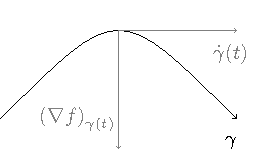
\includegraphics{figures/niveau}
  \caption{Eine Niveaulinie}%
  \label{fig:niveau}
\end{figure}

\begin{example}
  Betrachte die Funktion
  \begin{align*}
    f \colon \mathbb{R}^2 & \to \mathbb{R} \\
    p & \mapsto \langle p, p \rangle
  \end{align*}
  und die Kurve
  \begin{align*}
    \gamma \colon \mathbb{R} & \to \mathbb{R}^2 \\
    t & \mapsto (\cos(t), \sin(t)).
  \end{align*}
  Es gilt für alle $t \in \mathbb{R}$,
  dass
  \[
  \langle {(\nabla f)}_{\gamma(t)}, \dot \gamma(t) \rangle
  = \langle 2 \gamma(t), \dot \gamma(t) \rangle = 0.
  \]
  Tatsächlich sind die Kurven
  \begin{align*}
    \gamma_r \colon \mathbb{R} & \to \mathbb{R}^2 \\
    t & \mapsto (r\cos(t), r\sin(t))
  \end{align*}
  für alle $r > 0$ Niveaulinien von $f$.
\end{example}

\subsubsection*{Der Mittelwertsatz}
Sei $a, b \in \mathbb{R}^n$ mit $a \neq b$.
Definiere $I_{a, b} = \left\{a + t(b-a) \mid t \in [0, 1]\right\}$.
Die Menge $I_{a, b}$ besteht aus allen Punkten die auf dem Geradenabschnitt
zwischen $a$ und $b$ liegen.

\begin{theorem}[Mittelwertsatz]
  Sei $f \colon \mathbb{R}^n \to \mathbb{R}$ differenzierbar
  und $a, b \in \mathbb{R}^n$ mit $a \neq b$.
  Dann existiert $p \in I_{a, b} \setminus \{a, b\}$ mit
  \[
    {(Df)}_p(b-a) = f(b) - f(a).
  \]
\end{theorem}

\begin{specialcases}
  \leavevmode
  \begin{enumerate}[(i)]
    \item Sei $f \colon \mathbb{R} \to \mathbb{R}$ (das heisst $n = 1$).
      Seien $a, b \in \mathbb{R}$ mit $a < b$.
      Dann existiert $x \in I_{a, b} \setminus \{a, b\} = (a, b)$ 
      mit ${(Df)}_{x(b-a) = f(b) - f(a)}$.
      Es gilt also
      \[
        f'(x) = \frac{f(b) - f(a)}{b-a}.
      \]
      Wir haben also die eindimensionale Version des Mittelwertsatzes
      erfolgreich aus der momentanen Version extrahiert.
    \item Nehme an, dass  $f(b) = f(a)$ gilt.
      Dann existiert $p \in I_{a, b} \setminus \{a, b\}$ 
      mit
      \[
        \langle {(\nabla f)}_{p}, b-a \rangle
        = {(Df)}_p(b-a) = 0,
      \]
      das heisst ${(\nabla f)}_p$ steht senkrecht auf $b-a$.
      Betrachte zum Beispiel
      \begin{align*}
        f \colon \mathbb{R}^2 & \to \mathbb{R} \\
        p & \mapsto \langle p, p \rangle
      \end{align*}
      und seien $a, b \in \mathbb{R}^2$ mit $\Vert a \Vert_2 = \Vert b \Vert_2$.
      Für $p = (a + b)/2$ gilt dann
      ${(\nabla f)}_p = 2p$, was senkrecht auf $b - a$ steht.
  \end{enumerate}
\end{specialcases}

\begin{proof}[Beweis des Mittelwertsatzes]
  Wir leiten das Resultat aus dem Satz von Rolle aus der
  Analysis I her.
  Betrachte die Hilfsfunktion
  \begin{align*}
    h \colon [0, 1] & \to \mathbb{R} \\
    t & \mapsto f(a + t(b-a)) - f(a) - t(f(b) - f(a)).
  \end{align*}
  Berechne
  \[
    h (0) = h(1) = 0.
  \]
  Für alle $t \in (0, 1)$ gilt dank der Kettenregel, dass
  \[
    h'(t) = {(Df)}_{a + t(b-a)}(b-a) - (f(b) - f(a)),
  \]
  da ${(Df)}_{\gamma(t)}(\dot \gamma(t)) = {(Df)}_{a + t(b-a)}(b-a)$.
  Nach dem Satz von Rolle existiert $t_0 \in (0, 1)$ 
  mit $h'(t_0) = 0$.
  Setze $p = a + t_0(b-a) \in I_{a, b} \setminus \{a, b\}$.
  Dann gilt
  \[
    0 = h'(t_0) = {(Df)}_{a + t_0(b-a)}(b-a) - (f(b) - f(a)).
  \]
  Es folgt, dass ${(Df)}_p(b-a) = f(b) - f(a)$.
\end{proof}

\subsubsection*{Diffeomorphismen}
\begin{definition}
  Eine differenzierbare bijektive Abbildung
  $f \colon \mathbb{R}^n \to \mathbb{R}^n$ 
  heisst \emph{Diffeomorphismus}, falls $f$ 
  eine differenzierbare Umkehrabbildung $g \colon \mathbb{R}^n \to \mathbb{R}^n$ 
  hat.
  Das heisst, dass $g \circ f = f \circ g = \text{Id}_{\mathbb{R}^n}$.
\end{definition}

Für einen Diffeomorphismus $f \colon \mathbb{R}^n \to \mathbb{R}^n$ 
mit Umkehrabbildung $g$ erhalten wir dann
\[
  {(Dg)}_{f(p)} \circ {(Df)}_p 
  = {(D \text{Id}_{\mathbb{R}^n})}_p = \text{Id}_{\mathbb{R}^n}.
\]
Ähnlich gilt auch ${(Df)}_p \circ {(Dg)}_{f(p)} = \text{Id}_{\mathbb{R}^n}$ 
Folglich sind die linearen Abbildungen
${(Df)}_p$ und ${(Dg)}_{f(p)}$ zueinander
inverse Vektorraumisomorphismen von $\mathbb{R}^n$.
Insbesondere gilt
$\det {(Df)}_p \neq 0$.

\section{Der Umkehrsatz}
In~\cite{heuser} ist der Umkehrsatz im Abschnitt 171 diskutiert.
Wir haben oben gesehen, dass Differentiale differenzierbare Abbildungen
mit differenzierbarer Umkehrfunktion Vektorraumisomorphismen sind.
In diesem Abschnitt werden wir die Umkehrung dieser Aussage
untersuchen.

\begin{example}
  Sei $A \colon \mathbb{R}^n \to \mathbb{R}^n$ linear
  mit $\det(A) = \det({(DA)}_p) \ne 0$.
  Dann ist $A$ eine differenzierbare Funktion
  mit differenzierbarer Umkehrabbildung $A^{-1}$.
\end{example}

Wir erinnern uns nun an ein eindimensionales Phänomen,
welches wir bereits in der Analysis I untersucht haben.
Sei $f \colon \mathbb{R} \to \mathbb{R}$ 
differenzierbar mit $f'(x) > 0$ für alle $x \in \mathbb{R}$.
Dann ist $f$ injektiv.
Tatsächlich gilt für alle $a, b \in \mathbb{R}$ mit $a < b$,
dass
\[
  f(b) - f(a) = \int_{a}^{b} f'(x) \, dx > 0.
\]
Insbesondere gilt $f(b) \neq f(a)$.

\begin{question}
  Sei $f \colon \mathbb{R}^n \to \mathbb{R}^n$ stetig
  differenzierbar, so dass für alle
  $p \in \mathbb{R}^n$ gilt, dass
  das Differential ${(Df)}_p$ in allen Punkten
  $p \in \mathbb{R}^n$ ein Isomorphismus ist, das heisst
  $\det({(Df)}_p) \neq 0$.
  Ist dann $f$ injektiv?
\end{question}

Die Antwort dazu ist nein, wie folgendes Beispiel zeigt.

\begin{example}
  Betrachte die \emph{komplexe Exponentialfunktion}
  \begin{align*}
    f \colon \mathbb{R}^2 & \to \mathbb{R}^2 \\
    (x, y) & \mapsto (e^{x} \cos y, e^x \sin y).
  \end{align*}
  Dann ist $f$ stetig differenzierbar, da die Komponentenfunktionen
  $f_1(x, y) = e^{x} \cos y$ und $f_2(x, y) = e^x \sin y$ 
  differenzierbar sind. Das folgt aus Betrachtungen in
  der Analysis I und der Produktregel.
  Berechne für $p = (x, y)$ die Jakobimatrix
  \[
    {(Jf)}_p =
    \begin{pmatrix}
      \frac{\partial f_1}{\partial x} & \frac{\partial f_1}{\partial y} \\
      \frac{\partial f_2}{\partial x} & \frac{\partial f_2}{\partial y}
    \end{pmatrix}
    =
    \begin{pmatrix}
      e^y \cos y & - e^x \sin y \\
      e^x \sin y & e^x \cos y
    \end{pmatrix}.
  \]
  Aus $\cos^2 + \sin^2 = 1$ folgt, dass $\det({(Jf)}_p) = e^x > 0$ 
  für alle $p = (x, y)$.
  Aber $f$ ist nicht injektiv, da $f(x, y) = f(x, y + 2 \pi)$ gilt.
\end{example}

\subsection*{Stetige Differenzierbarkeit}
Sei $U \subset \mathbb{R}^n$ offen und
$f \colon U \to \mathbb{R}^m$ differenzierbar.
Dann erhalten wir für alle $p \in U$ eine lineare
Abbildung ${(Df)}_p \colon \mathbb{R}^n \to \mathbb{R}^m$,
das heisst, dass ${(Df)}_p \in \text{Hom}(\mathbb{R}^n, \mathbb{R}^m)$,
wobei $\text{Hom}(\mathbb{R}^n, \mathbb{R}^m)$ aus
allen linearen Abbildungen $L \colon \mathbb{R}^n \to \mathbb{R}^m$ besteht.
Auf $\text{Hom}(\mathbb{R}^n, \mathbb{R}^m)$ haben wir
eine Norm, nämlich die Operatornorm $\Vert \cdot \Vert_{\text{op}}$.

\begin{definition}
  Sei $U \subset \mathbb{R}^n$ offen.
  Eine Abbildung $f \colon U \to \mathbb{R}^m$ heisst
  \emph{stetig differenzierbar} oder $C^1$,
  falls $f$ differenzierbar ist, und die Abbildung
  \begin{align*}
    df \colon U & \to \text{Hom}(\mathbb{R}^n, \mathbb{R}^m) \\
    p & \mapsto {(Df)}_p
  \end{align*}
  bezüglich der Operatornorm auf $\text{Hom}(\mathbb{R}^n, \mathbb{R}^m)$ 
  stetig ist.
  Ausgepackt heisst das, dass für alle $p \in U$ 
  und alle $\varepsilon > 0$ ein $\delta > 0$ 
  existiert, so dass
  \begin{enumerate}[(i)]
    \item $B_p(\delta) \subset U$, 
    \item für alle $q \in B_p(\delta)$ gilt, dass
      $\Vert {(Df)}_q - {(Df)}_p \Vert_{\text{op}} \leq \varepsilon$.
  \end{enumerate}
\end{definition}

In Koordinaten heisst das, dass die Einträge der
Jakobimatrix ${(Jf)}_p \in \mathbb{R}^{m \times n}$ stetig
von $p$ abhangen.
In anderen Worten ist für alle $i \leq m$ und $j \leq n$ 
die partielle Ableitungsfunktion
\begin{align*}
  \frac{\partial f_i}{\partial x_j} \colon U & \to \mathbb{R} \\
  p & \mapsto \frac{\partial f_1}{\partial x_j}(p)
  = \lim_{t \to 0} \frac{f_i(p + te_j) - f_i(p)}{t}
\end{align*}
stetig.

\begin{remarks}
  \leavevmode
  \begin{enumerate}[(1)]
    \item Die Existenz der partiellen Ableitungsfunktionen
      reicht nicht, um die Differenzierbarkeit von $f$ zu garantieren.
      Das Beispiel dazu war die Funktion
      \begin{align*}
        f \colon \mathbb{R}^2 & \to \mathbb{R} \\
        (x, y) & \mapsto 
        \begin{cases}
          0 & (x, y) = (0, 0),\\
          \frac{xy}{x^2 + y^2} & (x, y) \neq (0, 0).
        \end{cases}
      \end{align*}
      Diese Funktion $f$ hat in allen Punkten $p = (x, y)$ partielle
      Ableitungen, ist aber nicht einmal stetig bei $p = (0, 0)$.
    \item Es existiert dennoch ein Differenzierbarkeitskriterium,
      welches auf der Stetigkeit der partiellen Ableitungen beruht.
  \end{enumerate}
\end{remarks}

\begin{proposition}\label{prop:continuous-partial-derivatives}
  Sei $U \subset \mathbb{R}^n$ offen und
  $f \colon U \to \mathbb{R}$ eine Abbildung,
  so dass für alle $j \leq n$ und alle $p \in U$ 
  die partielle Ableitung $\partial f/ \partial x_j (p) \in \mathbb{R}$ 
  existiert, und die Funktion
  \begin{align*}
    \frac{\partial f}{\partial x_j} \colon U & \to \mathbb{R} \\
    p & \mapsto \frac{\partial f}{\partial x_j}(p)
  \end{align*}
  stetig ist.
  Dann ist $f$ stetig differenzierbar und insbesondere differenzierbar.
\end{proposition}

Wir werden Proposition~\ref{prop:continuous-partial-derivatives}
nicht beweisen. Der Beweis kann
in~\cite{heuser} bei 163.1 nachgeschlagen werden.

\begin{examples}
  \leavevmode
  \begin{enumerate}[(1)]
    \item Alle polynomialen Abbildungen $f \colon \mathbb{R}^n \to \mathbb{R}$ 
      haben stetige partielle Ableitungen, sind also
      stetig differenzierbar.
    \item Die Funktion
      \begin{align*}
        f \colon \mathbb{R}^2 & \to \mathbb{R}^2 \\
        (x, y) & \mapsto (e^x \cos y, e^x \sin y)
      \end{align*}
      hat stetige partielle Ableitungen und ist somit stetig
      differenzierbar.
  \end{enumerate}
\end{examples}

\begin{proposition}[Lokale Injektivität]\label{prop:local-injectivity}
  Sei $U \subset \mathbb{R}^n$ offen,
  $f \colon U \to \mathbb{R}$ stetig differenzierbar,
  und $p \in U$ so dass
  ${(Df)}_p \colon \mathbb{R}^n \to \mathbb{R}^n$ 
  ein Isomorphismus ist.
  Dann existiert $\varepsilon > 0$ mit
  \begin{enumerate}[\normalfont(i)]
    \item $B_p(\varepsilon) \subset U$,
    \item die Einschränkung von $f$ auf $B_p(\varepsilon)$ ist
      injektiv.
  \end{enumerate}
\end{proposition}

\begin{proof}
  Nach Annahme ist $A = {(Df)}_p$ ein Isomorphismus.
  Betrachte $f$ die Komposition
  $\overline f = A^{-1} \circ f \colon U \to \mathbb{R}^n$.
  Für alle $q \in U$ 
  gilt nach der Kettenregel, dass
  \[
    {(D \overline f)}_q = {(DA^{-1})}_{f(q)} \circ {(Df)}_q
    = A^{-1} \circ {(Df)}_q.
  \]
  In anderen Worten ist $\overline f$ auch stetig differenzierbar
  und es gilt
  \(
    {(D \overline f)}_p = \text{Id}_{\mathbb{R}^n}.
  \)

  Wähle nun $\varepsilon > 0$ so, dass
  \begin{enumerate}[(i)]
    \item $B_p(\varepsilon) \subset U$,
    \item für alle $q \in B_p(\varepsilon)$ gilt, dass
      \(
        \Vert {(D \overline f)}_q - {(D \overline f)}_p \Vert_{\text{op}}
          \leq 1/2
      \).
  \end{enumerate}
  Wir behaupten nun, dass die Einschränkung
  $ \overline f |_{B_p(\varepsilon)} \colon B_p(\varepsilon) \to \mathbb{R}^n$ 
  injektiv ist.
  Daraus wird folgen, dass $f |_{B_p(\varepsilon)} = A \circ
  \overline f |_{B_p(\varepsilon)}$ auch injektiv ist, da $A$ selbst
  bijektiv ist.
  Es bleibt also lediglich die Behauptung zu zeigen.

  Dazu seien $q, \widetilde q \in B_{p}(\varepsilon)$ 
  mit $q \neq \widetilde q$.
  Wir wollen zeigen, dass $ \overline f(\widetilde q) \neq  \overline f(q)$.
  Dazu betrachte die Kurve
  \begin{align*}
    \gamma \colon [0, 1] & \to B_p(\varepsilon) \\
    t & \mapsto q + t(\widetilde q - q).
  \end{align*}
  Definiere eine Hilfsabbildung
  \begin{align*}
    h \colon [0, 1] & \to \mathbb{R}^n \\
    t & \mapsto \overline f (\gamma(t)) = \overline f(q + t(\widetilde q - q)).
  \end{align*}
  Dann ist $h$ eine differenzierbare Kurve mit
  \[
    h'(t) = {(D\overline f)}_{\gamma(t)}(\dot \gamma(t))
    = {(D \overline f)}_{q + t(\widetilde q - q)}( \widetilde q - q) \in \mathbb{R}^n.
  \]
  Berechne nun mithilfe dem Integralsatz
  für Kurven, dass
  \[
      \overline f(\widetilde q) -  \overline f(q) 
     = h(1) - h(0) 
     =\int_{0}^{1} h'(t) \, dt
    = \int_{0}^{1} {(D \overline f)}_{q + t(\widetilde q - q)}(\widetilde q - q) \, dt.
  \]
  Berechne nun
  \begin{align*}
    \overline f(\widetilde q) - \overline f(q)
    & = \int_{0}^{1} {(D \overline f)}_p (\widetilde q - q) \, dt
    + \int_{0}^{1} {(D \overline f)}_{q + t(\widetilde q - q)}
    (\widetilde q - q) - {(D \overline f)}_p (\widetilde q - q)\, dt\\
    &= \widetilde q - q + R,
  \end{align*}
  wobei
  \[
    R = \int_{0}^{1} {(D \overline f)}_{q + t(\widetilde q - q)}
     (\widetilde q - q) - {(D \overline f)}_p (\widetilde q - q)\, dt.
  \]
  Schätze ab, dass
  \[
    \Vert R \Vert_2
    \leq \int_{0}^{1} \Vert {(D \overline f)}_{q + t(\widetilde q - q)}
    (\widetilde q - q) - {(D \overline f)}_p (\widetilde q - q)\Vert_2 \, dt.
  \]
  Für alle $t \in [0, 1]$ gilt nach Wahl von $\varepsilon$,
  dass
  \(
    \Vert {(D \overline f)}_{\gamma (t)} - {(D \overline f)}_p \Vert_{\text{op}} \leq 1/2
  \)
  gilt, da $\gamma(t) \in B_p(\varepsilon)$.
  Es folgt, dass
  \(
    \Vert {(D \overline f)}_{\gamma(t)}
    (\widetilde q - q) - {(D \overline f)}_p (\widetilde q - q)\Vert_2 
    \leq 1/2 \cdot \Vert \widetilde q - q \Vert_2,
  \)
  also auch
  \[
    \Vert R \Vert_2 \leq \int_{0}^{1} \frac{1}{2} \cdot
    \Vert \widetilde q - q \Vert_2 \, dt
    \leq \frac{1}{2} \cdot \Vert \widetilde q - q \Vert_2.
  \]
  Aus $\overline f (\widetilde q ) - \overline f(q) = \widetilde q - q + R$ 
  mit $\Vert R \Vert_2 \leq 1/2 \cdot \Vert \widetilde q - q \Vert_2$
  folgt, dass
   \[
     \Vert \overline f (\widetilde q ) - \overline f(q) \Vert_2 \geq
     1/2 \cdot \Vert \widetilde q - q \Vert_2,
  \]
  und insbesondere ist $\overline f (\widetilde q ) \neq \overline f ( q)$.
\end{proof}

\begin{theorem}[Umkehrsatz]
  Sei $U \subset \mathbb{R}^n$ offen, $f \colon U \to \mathbb{R}^n$ 
  stetig differenzierbar, und $p \in U$ ein Punkt mit
  $\det( {(Df)}_p ) \neq 0$.
  Dann existieren offene Mengen $V, W \subset \mathbb{R}^n$
  mit 
  $p \in V \subset U$ und
  $f(p) \in W$,
  sowie eine differenzierbare Abbildung $g \colon W \to V$ mit
  $f \circ g = \text{Id}_W$ und $g \circ f|_V = \text{Id}_V$.
  Für alle $y \in W$ gilt ${(Dg)}_y = {(Df)}_{g(y)}^{-1}$.
\end{theorem}

\begin{figure}[htb]
  \centering
  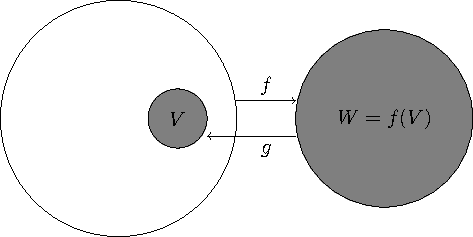
\includegraphics{figures/inversefunction}
  \caption{Der Umkehrsatz}%
  \label{fig:inversefunction}
\end{figure}

Die einzelnen Schritte des Beweises sind folgende.
\begin{enumerate}[(1)]
  \item Lokale Injektivität (siehe 
    Proposition~\ref{prop:local-injectivity} oben),
  \item Lokale Surjektivität,
  \item Differenzierbarkeit der lokalen Umkehrfunktion $g \colon W \to V$.
\end{enumerate}

Um die beiden letzten Schritte des Beweises auszuführen,
treffen wir folgende Vorbereitungen.
\begin{enumerate}[(i)]
  \item Definiere
    \begin{align*}
      \overline f \colon U & \to \mathbb{R}^n \\
      q & \mapsto ({(Df)}_p^{-1} \circ f)(q).
    \end{align*}
    Dann gilt ${(D \overline f)}_p = {(Df)}_p^{-1} \circ {(Df)}_p 
    = \text{Id}_{\mathbb{R}^n}$.
    Wähle $\varepsilon > 0$ so, dass $B_p(\varepsilon) \subset U$,
    und so dass für alle $q \in B_p(\varepsilon)$ gilt, dass
    \(
      \Vert {(D \overline f)}_q - {(D \overline f)}_p \Vert_{\text{op}}
        \leq 1/2
    \).
    Für alle $q, \widetilde q \in B_p(\varepsilon)$ gilt dann, dass
    \[
      \overline f ( \widetilde q ) - f(q) = \widetilde q - q + R
    \]
    mit $\Vert R \Vert_2 \leq 1/2 \cdot \Vert \widetilde q - q \Vert_2$,
    wie im Beweis von Proposition~\ref{prop:local-injectivity}.
    Insbesondere gilt
    \[
      1/2 \cdot \Vert \widetilde q - q \Vert_2 \leq
      \Vert \overline f ( \widetilde q ) - \overline f (q) \Vert_2
      \leq 3/2 \cdot \Vert \widetilde q - q \Vert_2.
    \]
  \item Definiere $\widetilde U = U - p
    = \left\{q \in \mathbb{R}^n \mid q + p \in U\right\}$
    und 
    \begin{align*}
      \widetilde f \colon \widetilde U & \to \mathbb{R}^n \\
      q & \mapsto f(p + q) - f(p).
    \end{align*}
    Dann gilt $\widetilde f ( 0 ) = \overline f(p) - \overline f (p) = 0$.
    Weiterhin gilt ${(D\widetilde f )}_0 = \text{Id}_{\mathbb{R}^n}$.
    Dies fällt aus der Dreigliedentwicklung
    \[
      \widetilde f ( 0 + h ) = \widetilde f (h)
      = \overline f ( p + h ) - \overline f ( p )
      = {(D \overline f )}_p(h) + {(R \overline f)}_p (h)
    \]
    Wir werden nun mithilfe dieser Vereinfachungen annehmen,
    dass
    \begin{itemize}
      \item $p = 0$,
      \item $f(0) = 0$,
      \item ${(Df)}_0 = \text{Id}_{\mathbb{R}^n}$.
    \end{itemize}
\end{enumerate}

Mit dem $\varepsilon > 0$ aus dem Beweis von
Proposition~\ref{prop:local-injectivity} gilt,
dass
$f |_{B_0(\varepsilon)}$ injektiv ist.
In einem nächsten Schritt werden wir zeigen,
dass für das selbe $\varepsilon > 0$ auch gilt,
dass $B_0(\varepsilon/2) \subset f(B_0(\varepsilon))$,
das heisst, für alle $y \in \mathbb{R}^n$ 
mit $\Vert y \Vert_2 < \varepsilon/2$ existiert
ein $q \in \mathbb{R}^n$ mit $\Vert q \Vert_2 < \varepsilon$ 
und $f(q) = y$.
Nach dem ersten Schritt ist dieses $q \in B_0(\varepsilon)$ 
dann eindeutig. Wir werden es mit $g(y)$ bezeichnen.

Es stellt sich heraus, dass wir $g$ rekursiv definieren können.
Als nullten Ansatz wählen wir \[g_0(y) = y.\]
Da $f$ in erster Ordnung die Identität ist, sollte das
nicht allzu schlecht sein.
Der erste Ansatz ist dann $g_1(y) = g_0(y) + y - f(g_0(y))$.
Rekursiv setzen wir
\[
  g_{n+1}(y) = g_n(y) + y - f(g_n(y)).
\]

\begin{remark}
  Falls per Zufall $f(g_n(y)) = y$ für ein $n \in \mathbb{N}$ 
  gilt, dann folgt auch, dass
  \(
    g_{n+1}(y) = g_n(y)
  \).
  Insbesondere ist auch $f(g_{n+1}(y)) = y$.
\end{remark}

\begin{claim}[Lokale Surjektivität]
  Der Grenzwert $g(y) = \lim_{n \to \infty} g_n(y) \in B_{0}(\varepsilon)$ 
  existiert, und $f(g(y)) = y$.
\end{claim}

\begin{proof}
  Durch vollständige Induktion zeigen wir
  \begin{enumerate}[(i)]
    \item $\Vert g_n(y) \Vert_2 < (1 - 1/2^{n+1}) \cdot \varepsilon$ 
    \item $\Vert g_{n+1}(y) - g_n(y) \Vert_2 < \varepsilon / 2^{n+2}$.
  \end{enumerate}
  Für $n = 0$ stimmt diese Behauptung, da
  \[
    \Vert g_0(y) \Vert_2 = \Vert y \Vert_2 < \varepsilon / 2 = (1 - 1/2)
    \cdot \varepsilon
  \]
  und
  \[
    \Vert g_1(y) - g_0(y) = \Vert y - f ( g_0(y)) \Vert_2
    = \Vert y - f(y) \Vert_2 \leq \Vert R \Vert_2
    \leq \Vert y \Vert_2 / 2 < \varepsilon / 4,
  \]
  wobei $R$ in der Vorbereitung (i) untersucht wurde.
  Für den Induktionsschritt, berechne
  \begin{align*}
    \Vert g_{n+1}(y) \Vert_2 
    &\leq  \Vert g_n(y) \Vert_2 + \Vert g_{n+1}(y) - g_n(y) \Vert_2 \\
    &\leq (1 - 1/2^{n+1}) \cdot \varepsilon
    + \varepsilon / 2^{n+2} = (1 - 1/2^{n+2}) \varepsilon.
  \end{align*}
  Ähnlich berechne
  \begin{align*}
    \Vert g_{n+2}(y) - g_{n+1}(y) \Vert_2 
    &= \Vert g_{n+1}(y) - f(g_{n+1}(y)) - g_n(y) + f(g_n(y)) \Vert_2  \\
    &= \Vert g_{n+1}(y) - g_n(y) - (f(g_{n+1}(y)) - f(g_n(y))) \Vert_2 \\
    &\leq 1/2 \Vert g_{n+1}(y) - g_n(y) \Vert_2 \\
    &< 1/2 \cdot \varepsilon \cdot 1/2^{n+2} = 1/2^{n+3}.
  \end{align*}
  Hier haben wir die Abschätzung aus der Vorbereitung (i)
  sowie die Induktionsannahme verwendet.

  Wir folgern, dass $(g_n(y))_{n \in \mathbb{N}}$ eine Cauchyfolge in
  $B_0(\varepsilon)$ ist.
  Wir schätzen ab, dass
  \begin{align*}
    \Vert g(y) \Vert_2
    & \leq \Vert g_0(y) \Vert_2 +
    \Vert g_1(y) - g_0(y) \Vert_2
    + \Vert g_2(y) - g_1(y) \Vert_2 + \cdots \\
    &< \varepsilon/2 + \varepsilon/4 + \varepsilon/8 + \cdots \\
    &= \varepsilon,
  \end{align*}
  also liegt $g(y)$ in $B_0(\varepsilon)$.
  Berechne nun mithilfe der Stetigkeit von $f$, dass
  \begin{align*}
    f(g(y))
    & = f \left( \lim_{n \to \infty}g_n(y) \right)\\
    &= \lim_{n \to \infty} f(g_n(y)).
  \end{align*}
  Aus $g_{n+1}(y) = g_n(y) + y - f(g_n(y))$ folgt, dass
  \begin{align*}
    f(g(y)) 
    &= \lim_{n \to \infty} y + g_n(y) - g_{n+1}(y)  \\
    &= y + g(y) - g(y) = y. \qedhere
  \end{align*}
\end{proof}

Im letzten Schritt des Beweis vom Umkehrsatz zeigen wir,
dass die oben konstruierte Umkehrfunktion $g$ differenzierbar ist.
Betrachte dazu die beiden Mengen $W = B_0(\varepsilon / 2)$ und 
$V = f^{-1}(W) \cap B_0(\varepsilon) \subset U$.
Aus der lokalen Bijektivität folgt, dass die Einschränkung
$f|_{V} \colon V \to W$ bijektiv ist, mit Umkehrabbildung
$g \colon W \to V$.

\begin{claim}
  Die Abbildung $g \colon W \to V$ ist Lipschitz-stetig
  mit Konstante $2$.
\end{claim}

\begin{proof}
  Für alle $q, \widetilde q \in B_0(\varepsilon)$ gilt
  \(
    1/2 \cdot 
    \Vert \widetilde q - q \Vert_2 \leq f(\widetilde q) - f(q) \Vert_2.
  \)
  Seien nun $\widetilde y, y \in W$. Setze
  $\widetilde q = g(\widetilde y)$ 
  und $q = g(y) \in V$.
  Es folgt, dass
  \[
    1/2 \cdot \Vert g(\widetilde y) - g(y) \Vert_2 \leq
    \Vert f(g(\widetilde y )) - f(g(y)) \Vert_2 = \Vert \widetilde y
    - y \Vert_2,
  \]
  was $\Vert g( \widetilde y ) - g(y) \Vert_2 \leq 2 \cdot \Vert \widetilde
  y - y \Vert_2$
  impliziert.
\end{proof}

Sei $y \in W$ und $k \in \mathbb{R}^n$ mit $y + k \in W$.
Betrachte den Ansatz
\[
  g(y + k ) = g(y) + {(Df)}_{g(y)}^{-1}(k) + {(Rg)}_{y}(k).
\]
für eine Dreigliedentwicklung für $g$ an der Stelle $y$.
Zu zeigen ist, dass ${(Rg)}_{y}(k)$ relativ klein in $\Vert k \Vert_2$ ist,
dass heisst, dass
\[
  \lim_{\Vert k \Vert_2 \to 0}
  \frac{\Vert {(Rg)}_y(k) \Vert_2}{\Vert k \Vert_2} = 0.
\]
Nach Konstruktion von $\varepsilon > 0$ gilt für
$g(y) \in V$, dass
\[
  \Vert {(Df)}_g(y) - {(Df)}_0 \Vert_{\text{op}} \leq 1/2,
\]
wobei ${(Df)}_0 = \text{Id}_{\mathbb{R}^n}$.
Es gilt also für alle $v \in \mathbb{R}^n$, dass
\(
  \Vert {(Df)}_{g(y)}(v) - v \Vert_2 \leq 1/2 \cdot \Vert v \Vert_2.
\)
Wir schliessen, dass $1/2 \cdot \Vert v \Vert_2 \leq \Vert
{(Df)}_{g(y)}(v) \Vert_2$.
Insbesondere ist ${(Df)}_{g(y)}$ invertierbar.

Sei nun $w \in \mathbb{R}^n$. Für  $v = {(Df)}_{g(y)}^{-1}(w)$ erhalten
wir, dass
\[
  1/2 \cdot \Vert {(Df)}^{-1}_{g(y)}(w) \Vert_2
  \leq \Vert {(Df)}_{g(y)}({(Df)}_{g(y)}^{-1}(w)) \Vert_2 = \Vert w \Vert_2,
\]
beziehungsweise 
$\Vert {(Df)}_{g(y)}^{-1}(w) \Vert_2 \leq 2 \cdot \Vert w \Vert_2$.
Folglich gilt $\Vert {(Df)}^{-1}_{g(y)} \Vert_{\text{op}} \leq 2$.
Wende nun auf unseren Ansatz die Abbildung $f$ auf beide Seiten an.
Die Linke seite wird dann zu $f(g(y + k)) = y + k$,
und die rechte Seite zu $f(g(y) + h)$,
wobei $h = {(Df)}^{-1}_{g(y)}(k) + {(Rg)}_y(k)$.
Es gilt
\[
  \Vert h \Vert \leq \Vert g(y + k ) - g(y) \Vert_2
  \leq 2 \cdot \Vert k \Vert_2.
\]
Die Dreigliedentwicklung von $f$ bei $g(y)$ liefert, dass
\begin{align*}
   f(g(y) + h) 
   & = f(g(y)) + {(Df)}_{g(y)}(h) + {(Rf)}_{g(y)}(h) \\
   &= y + {(Df)}_{g(y)}({(Df)}_{g(y)}^{-1}(k) + {(Rg)}_y(k))  
   + {(Rf)}_{g(y)}(h)\\
   &= y + k + {(Df)}_{g(y)}({(Rg)}_y(k)) + {(Rf)}_{g(y)}(h).
\end{align*}
Hier haben wir verwendet, dass ${(Df)}^{-1}_{g(y)}$ linear ist.
Gleichsetzen der beiden Seiten liefert, dass
\(
  y+ k
  = y + k + {(Df)}_{g(y)}({(Rg)}_{y}(k)) + {(Rf)}_{g(y)}(h),
\)
also gilt
\[
  {(Rg)}_y(k) = - {(Df)}_{g(y)}^{-1}({(Rf)}_{g(y)}(h)).
\]
Aus $\Vert {(Df)}^{-1}_{g(y)} \Vert_{\text{op}} \leq 2$ 
folgt, dass $\Vert {(Rg)}_y(k) \Vert_2
\leq 2 \cdot \Vert {(Rf)}_{g(y)}(h) \Vert_2$ gilt.
Wir schliessen, dass
\begin{align*}
  \lim_{\Vert k \Vert_2 \to 0}
  \frac{\Vert {(Rg)}_y(k) \Vert_2}{\Vert k \Vert_2}
  &\leq \lim_{\Vert k \Vert_2 \to 0} 2 \cdot
  \frac{\Vert {(Rf)}_{g(y)}(h) \Vert_2}{\Vert k \Vert_2}\\
  &\leq \lim_{\Vert h \Vert_2 \to 0}
  4 \cdot \frac{\Vert {(Rf)}_{g(y)}(h) \Vert_2}{\Vert h \Vert_2}  = 0,
\end{align*}
da ${(Rf)}_{g(y)}(h)$ relativ klein in $\Vert h \Vert_2$ ist.
Wir haben hier verwendet, dass $\Vert h \Vert_2 \leq 2 \cdot \Vert k \Vert_2$ 
gilt, um $\Vert k \Vert_2 \to 0$ durch $\Vert h \Vert_2 \to 0$ zu ersetzen.
Wir folgern, dass obiger Ansatz tatsächlich
eine Dreigliedentwicklung von $g$ an der Stelle $y \in W$ ist.
Somit ist $g$ differenzierbar, und für alle
$y \in W$ gilt, dass
${(Dg)}_y = {(Df)}_{g(y)}^{-1}$.

Wir werden darauf verzichten, 
die Transformationen, welche wir zu Beginn auf $f$ angewendet haben,
wieder rückgängig zu machen (obwohl das nicht allzu schwierig wäre).
Somit ist der Umkehrsatz vollständig bewiesen.

\begin{remark}
  Die stetige Differenzierbarkeit von $f$ 
  ist eine essentielle Hypothese im Umkehrsatz,
  bereits in einer Variable.
\end{remark}

\begin{example}
  Betrachte die Funktion
  \begin{align*}
    f \colon \mathbb{R} & \to \mathbb{R} \\
    x & \mapsto 
    \begin{cases}
      0 & x = 0, \\
      x + 2x^2 \cdot \sin(1/x) & x \neq 0.
    \end{cases}
  \end{align*}
  Die Funktion $f$ ist differenzierbar, und es gilt
  \[
    f'(x) =
    \begin{cases}
      1 & x = 0, \\
      1 + 4x \cdot \sin(1/x) - 2 \cos(1/x) & x \neq 0.
    \end{cases}
  \]
  Für alle $x_n = 1/2\pi n$ gilt, dass $f'(x_n) = 1 + 0 - 2 = -1$ gilt.
  Also gilt
  \[
    \lim_{n \to \infty} f'(x_n) = -1 \neq 1 = f'(0)
    = f' \left( \lim_{n \to \infty} x_n \right).
  \]
  Also ist $f'$ an der Stelle $x = 0$ nicht stetig, und
  ausserdem in keiner noch so kleinen offenen Umgebung
  von $x = 0$ monoton wachsend.
  Insbesondere hat $f$ keine lokale Umkehrfunktion.
\end{example}

\section{Der Satz über implizite Funktionen}
In~\cite{heuser} wird der Satz über implizite Funktionen 
in den Abschnitten~169 und 170 diskutiert.
Der Beweis des Satzes empfiehlt sich nicht, dort nachzulesen.
Der Grund dazu ist, dass dort (und auch in den meisten
anderen Lehrbüchern) der 
Umkehrsatz aus dem Satz über implizite Funktionen
hergeleitet wird. Wir machen das in dieser Vorlesung umgekehrt. 

Sei $f \colon \mathbb{R}^n \to \mathbb{R}^m$ 
stetig differenzierbar mit $m < n$.
Für alle $p \in \mathbb{R}^n$ erhalten wir eine
lineare Abbildung ${(Df)}_p \colon \mathbb{R}^n \to \mathbb{R}^m$.
Die Dimensionsformel aus der linearen Algebra liefert
\[
  n = \dim \ker {(Df)}_p + \dim \im {(Df)}_p,
\]
wobei $\ker {(Df)}_p$ den Kern und
$\im {(Df)}_p$ das Bild von ${(Df)}_p$ bezeichnet.
Aus der Beobachtung, dass
$\dim \im {(Df)}_p \leq m < n$ folgt, dass
$\dim \ker {(Df)}_p \geq 1$.
Insbesondere kann ${(Df)}_p$ kein Vektorraumisomorphismus sein.
Wohlaber kann ${(Df)}_p \colon \mathbb{R}^n \to \mathbb{R}^m$ 
surjektiv sein.

Im Spezialfall $m = 1$, das heisst $f \colon \mathbb{R}^n \to \mathbb{R}$ 
ist die Bedingung, dass ${(Df)}_p \colon \mathbb{R}^n \to \mathbb{R}$
nicht die Nullabbildung ist, oder äquivalent, dass
${(\nabla f)}_p$ nicht der Nullvektor ist.
Noch konkreter ist $({Df})_p \colon \mathbb{R}^n \to \mathbb{R}$
surjektiv, genau dann wenn eine partielle Ableitung $\partial f \partial x_k$
in $p$ nicht null ist.

\begin{question}
  Wie verhält sich $f \colon \mathbb{R}^n \to \mathbb{R}$ 
  in der Nähe eines Punkts $p \in \mathbb{R}^n$ mit
  ${(\nabla f)}_p \neq 0$? Genauer: Wie sehen die 
  \emph{Niveaumengen}
  \[
    f^{-1}(w) = \left\{q \in \mathbb{R}^n \mid f(q) = w\right\}
    \subset \mathbb{R}^n
  \]
  in der Nähe eines Punkts $p \in \mathbb{R}^n$ 
  mit ${(\nabla f)}_p \neq 0$ aus?
\end{question}

\begin{examples}
  \leavevmode
  \begin{enumerate}[(1)]
    \item Betrachte die Funktion
      \begin{align*}
        f \colon \mathbb{R}^2 & \to \mathbb{R} \\
        (x, y) & \mapsto y.
      \end{align*}
      Für alle $p = (x, y) \in \mathbb{R}^2$ gilt, dass
      ${\nabla f}(p) = (0, 1) \neq 0$.
      Für $w \in \mathbb{R}$ ist
      \[
        f^{-1}(w) = \left\{(x, y) \in \mathbb{R}^2 \mid y = w\right\}.
      \]
      In anderen Worten sind alle horizontalen Geraden
      Niveaumengen.
    \item Betrachte die Funktion
      \begin{align*}
        f \colon \mathbb{R}^2 & \to \mathbb{R} \\
        (x, y) & \mapsto x^2 + y^2.
      \end{align*}
      Für $p = (x, y) \in \mathbb{R}^2$ gilt
      ${(\nabla f)}_p = 2p$.
      Also ist ${(\nabla f)}_p \neq 0$ für alle $p \neq 0$.
      Die Niveaumengen $f^{-1}(w)$ sind leer für negative $w$,
      der Nullpunkt für $w = 0$, und Kreise mit Radius $\sqrt w$ 
      für $w > 0$.
      Es fällt auf, dass die Niveaulinie Nullpunkt $w = 0$ 
      einer anderen Qualität ist, als die restlichen Niveaulinien.
      Es ist kein Zufall, dass genau in diesem Punkt der
      Gradient verschwindet.

    \item Betrachte die Funktion
      \begin{align*}
        f \colon \mathbb{R}^2 & \to \mathbb{R} \\
        (x, y) & \mapsto y^2 - x^2 = (y - x)(y + x).
      \end{align*}
      Für alle $p = (x, y) \in \mathbb{R}^2$ ist
      ${(\nabla f)}_p = (-2x, 2y)$ null, genau dann wenn $p$ 
      auch null ist.
      Für alle Werte $w \neq 0$ sind die
      Niveaulinien $f^{-1}(w)$ Hyperbeln.
      Insbesondere sehen sie wie
      differenzierbare Kurven aus.
      Aber bei $w = 0$ geschieht wieder
      etwas besonderes, nämlich ist
      die Niveaumenge $f^{-1}(0)$ 
      ein Kreuz, und nicht das
      Bild einer differenzierbaren Kurve.
  \end{enumerate}
\end{examples}

\begin{figure}[htb] 
  \centering
  \begin{minipage}{0.33\textwidth}
    \centering
    
\includegraphics{figures/niveauset1}
  \end{minipage}%
  \begin{minipage}{0.33\textwidth}
    \centering
    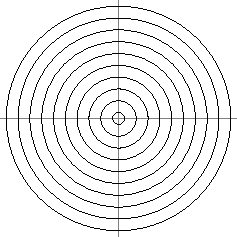
\includegraphics{figures/niveauset2}
  \end{minipage}%
  \begin{minipage}{0.33\textwidth}
    \centering
    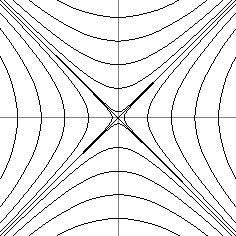
\includegraphics{figures/niveauset3}
  \end{minipage}%
  \caption{Die Niveaulinien aus den drei Beispielen}%
  \label{fig:niveausets}
\end{figure}

\begin{theorem}[Satz über implizite Funktionen, erste Version]
  Sei $f \colon \mathbb{R}^n \to \mathbb{R}$ 
  stetig differenzierbar und $p \in \mathbb{R}^n$ 
  so, dass ${(Df)}_p \colon \mathbb{R}^n \to \mathbb{R}$ surjektiv ist,
  das heisst, dass ${(\nabla f)}_p \neq 0$ ist.
  Nehme zusätzlich an, dass $p = 0$, $f(0) = 0$,
  und $\partial f/ \partial x_n (0) \neq 0$.
  Dann existieren $\varepsilon > 0$, $\delta > 0$,
  und eine differenzierbare Abbildung
  \[
  g \colon B_0^{\mathbb{R}^{n-1}}(\varepsilon) \times (-\delta, \delta)
  \to \mathbb{R},
  \]
  so dass für alle 
  $q = (x_1, \dots, x_{n-1}) \in B_0^{\mathbb{R}^{n-1}}(\varepsilon)$ 
  und alle $w \in (-\delta, \delta)$ gilt, dass
  \[
  f(x_1, \dots, x_{n-1}, g(x_1, \dots, x_{n-1}, w)) = w.
  \]
  Hier ist $B_0^{\mathbb{R}^{n-1}}(\varepsilon)
  = \left\{q \in\mathbb{R}^{n-1} \mid \Vert q \Vert_2 < \varepsilon \right\}$.
\end{theorem}

\begin{geometric}
  Bei festem $q = (x_1, \dots, x_{n-1}) \in B_0^{\mathbb{R}^{n-1}}$ 
  und festem $w \in (-\delta, \delta)$ hat die Gleichung
  $f(x_1, \dots, x_{n-1}, z) = w$ eine Lösung
  \[
  z = g(x_1, \dots, x_{n-1}, w) \in \mathbb{R}.
  \]
  Die Niveaumengen $f^{-1}(w)$ lassen sich in einer
  Umgebung des Punkts $p \in \mathbb{R}^n$ 
  als Graphen von Funktionen betrachten.
  Die Einschränkung von $g$ auf $B_0^{\mathbb{R}^{n-1}} \times \{w\}$
  liefert eine Abbildung
  \begin{align*}
    \overline g \colon B_0^{\mathbb{R}^{n-1}}(\varepsilon) & \to \mathbb{R} \\
    q & \mapsto g(q, w).
  \end{align*}
  Die Niveaulinie $f^{-1}(w)$ ist über
  $B_0^{\mathbb{R}^{n-1}}(\varepsilon)$ realisiert als Graph der
  Funktion $\overline g$.
\end{geometric}






\end{document}
